\chapter{ChIP-Seq项目实操}

本章将介绍ChIP-Seq的基本分析流程,包括上游分析和下游分析。\par
其中上游分析流程主要包括:
\begin{enumerate}
    \item fastq文件的质控、过滤、比对
    \item 比对文件的排序、过滤、去重、索引
    \item 查看ChIP-Seq分析的质量
\end{enumerate}

下游分析主要包括:
\begin{enumerate}
    \item call motif分析
    \item 与TSS的共定位分析
\end{enumerate}

本章涉及的软件较多,不能一一介绍其算法原理和详细的使用方法,因此对该项目代码中具体参数的调整需要争对不同的项目自行斟酌。但该项目代码依然具备较高的参考价值,可作为某些生信分析项目的通用分析模板。
感谢饶希晨师兄提供的大部分代码,我们在此基础上完成了后续代码的修改,并成功运行。\par
感谢李帅师兄的总结报告,为了该总结的完整性,我们在本章部分引用了李帅师兄的总结报告中的部分内容,如果对湿实验部分感兴趣,还请参考李帅的《生物信息技术期末总结》。


\section{背景介绍}

在此简要介绍该ChIP-Seq项目中使用到的一些基础概念。

\subsection{ChIP-Seq原理}

\textbf{染色质免疫共沉淀}(Chromatin Immunoprecipitation)实验主要用于目标蛋白会与基因组DNA中那些序列结合。其实验原理为,利用甲醛交联固定后,打断染色质DNA,与目标蛋白结合的DNA会与目标蛋白一起被目标蛋白的抗体免疫沉淀。\textbf{染色质免疫共沉淀测序技术}(ChIP-Seq)则是将上述免疫沉淀出的DNA接上测序接头,进行二代测序。
在此不再赘述湿实验的具体流程,本章主要聚焦该实验所得数据的生物信息学分析。ChIP-Seq的基本分析流程也可拓展应用到其他任何与\textbf{寻找目标核酸序列在基因组中的位置}相关的生信分析中。

\subsection{CTCF简介}
本章节使用的测序数据为CTCF蛋白的ChIP-Seq数据。\par
CCCTC-结合因子(CCCTC-binding factor, CTCF)是一种高度保守的锌指蛋白,可以作为转录激活因子、转录阻遏因子,此外还可以作为绝缘因子阻断增强子和启动子之间的通讯。\par
CTCF可以与染色质结构域边界结合的同时招募其他转录因子,并帮助真核基因组构建三维结构。\par
CTCF通过其11个锌指(ZF)定向结合众多CTCF结合位点(CBS)内的四个模块的特定序列元件,确定适当的全基因组染色质环相互作用。目前CTCF与CBS复合物的晶体结构已被解出。

\subsection{ChIP-Seq分析前的准备工作}
本项目的上游分析流程是许多生信分析共有的一般分析流程,包括质量控制、去接头、比对;比对文件的排序、转换、过滤、去重、索引。随后进行ChIP-Seq特有的分析,包括ChIP-Seq质量控制、富集峰的寻找。最后根据研究项目的目的可进行进一步下游分析,本项目进行了初步的下游分析,包括富集峰与转录起始位点(TSS)的共定位、峰基序分析(call motif)
\subsubsection{环境配置}

\begin{lstlisting}
    conda create -n chip-seq
    conda activate chip-Seq
    conda install fastqc 
    conda install cutadapt 
    conda install bowtie2 
    conda install samtools ## 操作比对结果文件的软件
    conda install macs2 ## 用于寻峰的软件
    conda install -c bioconda deeptools
    conda install -c idr ## 用于多样本合并的软件


    # meme套件和homer软件需要perl环境,建议编译安装perl环境后再编译安装上述软件
    # 下载meme套件安装包
    wget https://meme-suite.org/meme/meme-software/5.4.1/meme-5.4.1.tar.gz
    tar zxf meme-5.4.1.tar.gz
    cd meme-5.4.1
    ./configure --prefix=$HOME/meme --enable-build-libxml2 --enable-build-libxslt \par
    make
    make test
    make install

    wget http://homer.ucsd.edu/homer/configureHomer.pl
    perl configureHomer.pl -install
    Homer\_HOME=/Users/zhaohuanan/rxc/homer
    echo PATH="${Homer\_HOME}/bin:$PATH"
    chmod +x configureHomer.pl
    ./configureHomer.pl -install hg38


    # piacrd需要Java环境,建议安装openjdk
    sudo apt update 
    sudo apt install openjdk-17-jdk
    # 下载picard包,并添加至环境变量,http://broadinstitute.github.io/picard/
    java -jar /path/to/picard.jar -h 
    java -jar $PICARD -h 
    http://broadinstitute.github.io/picard/
\end{lstlisting}

\subsubsection{测序数据和参考文件的下载}
本项目使用的公共数据来自数据库ENCODE(DNA元件百科全书, Encyclopedia of DNA Elements) \par
项目数据的登录号为ENCSR617IFZ。实验数据总共有四个文件,分别是两个生物学重复的Read1和Read2,测序类型为双端101nt,文件格式为fastq。\par
其中生物学重复1测序数据注册号为ENCFF631JSV, ENCFF715KYL;生物学重复2的数据注册号为ENCFF002OWA, ENCFF833BQT。\par

\begin{figure}[ht]
    \centering
    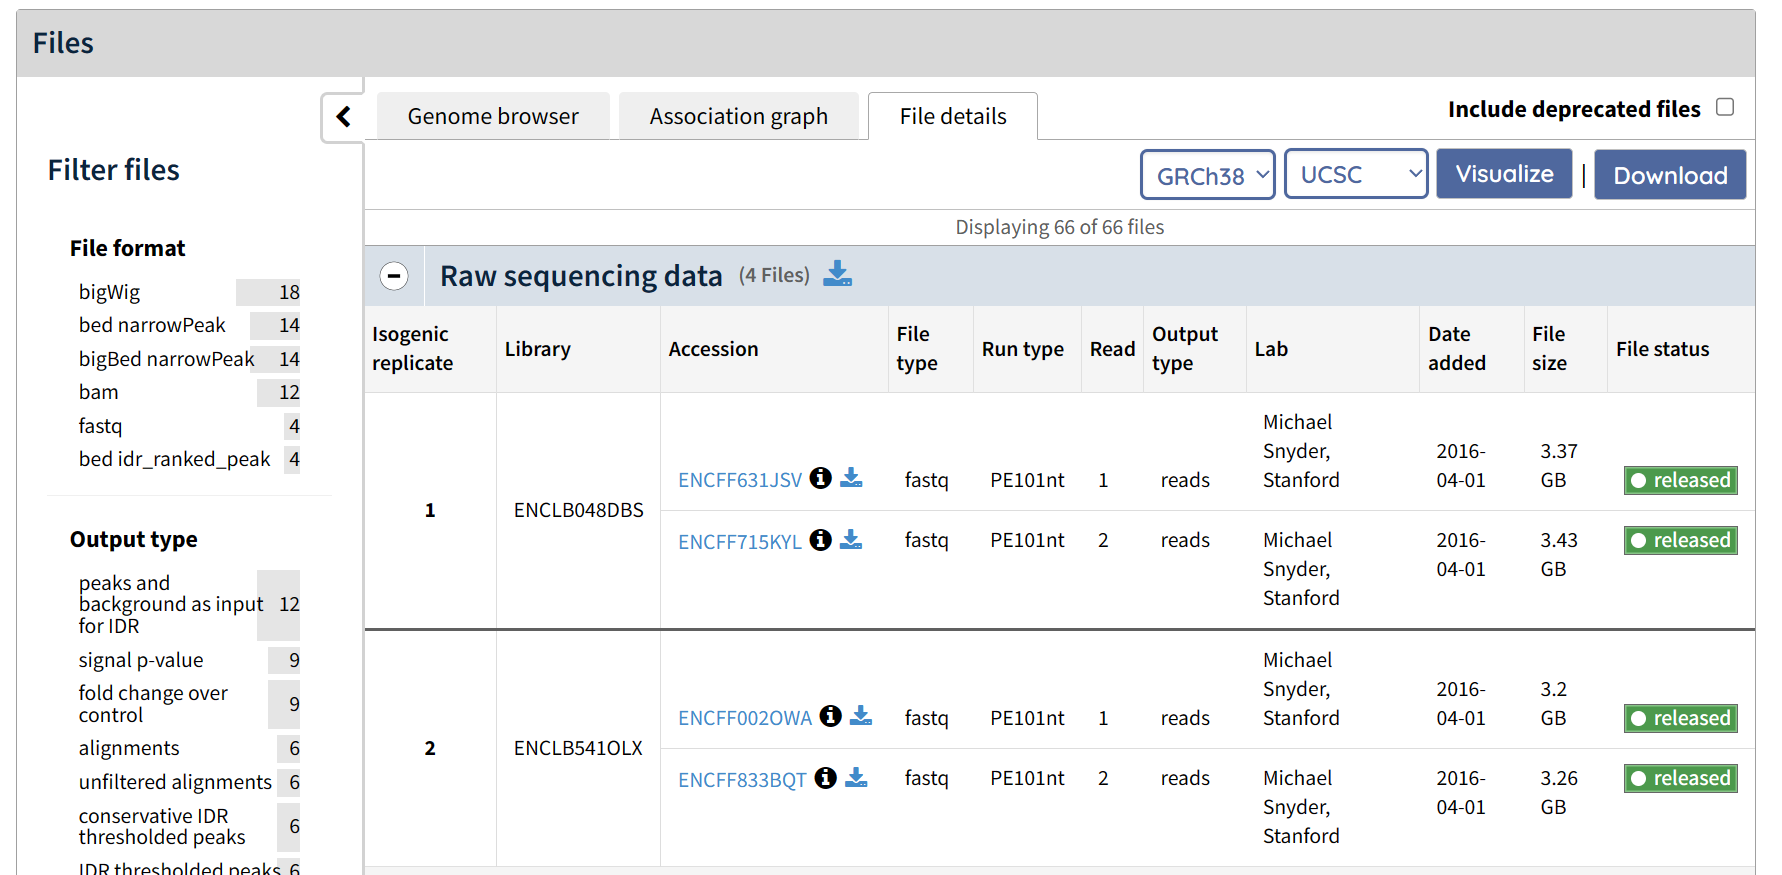
\includegraphics[width=10cm]{figure/encode_download.png}
\end{figure}
此外,在ChIP-Seq数据中寻找富集峰需要一份\textbf{未富集文库测序数据}作为参考(Input),本项目选用的数据注册号为:ENCFF873ZZU, ENCFF611URR.

\section{上游分析流程}
ChIP-Seq的一般分析流程
ChIP-Seq测序数据需要完成基本的NGS分析流程。该项目中,实验数据有两个生物学重复;此外为了call peak,另外需要一个未进行富集操作的测序数据作为参考。此三份数据采取完全相同的一般分析流程。\par
以本分析项目为例,作者希望建立一套尽可能自动化,规范化的流程。


\subsection{准备工作}
在分析开始之前,设置好自己的储存分配逻辑
\begin{lstlisting}
    #!/bin/bash

    ########
    # code for chipseq
    ########

    ##### 当前工作路径为 ##########
    ### 建议新建项目文件夹(此处为practice),并将该该文件夹设置为项目的工作路径
    # mkdir practice
    # cd practice
    # pwd
    # /home/wuhangrui/practice/

    ##### step0 创建原始数据与参考文件的软连接 #########
    ### 建议使用专门的存储空间或存储服务器存储原始数据和参考文件,并建议将其软链接到自己的工作路径下
    ## 在该项目的例子中,本章作者将下载的rawdata存放于nas中/nas\_data/whr/practice/chipseq/rawdata,
    ## 由于存储空间问题,本章作者在NAS中创建了存储中间结果的文件夹,并将该文件夹也软连接到工作目录下,以将中间结果文件也保存在NAS中
    ln -s /nas\_data/whr/practice/chipseq/ /home/wuhangrui/practice/chipseq
    cd ./chipseq

    # 创建存储中间结果的文件夹 
    mkdir 01\_fastqc 02\_cutadapt 03\_mapping 05\_peak\_calling

    # 读取样本名字
    cd ./rawdata

    # 把样本名字信息存放在config文件
    ls *\_r1.fastq.gz >config

    # 去掉后缀,仅保留名字信息
    sed -i "s/\_r1.fastq.gz//g" config

    cd /home/wuhangrui/practice/chipseq
\end{lstlisting}

\subsection{质量控制}
\begin{lstlisting}
    ##### step1 fastqc 质量控制 ##########
    ## 从nas里直接读取数据进行fastq,速度有点慢,建议在同一局域网下进行

    # 指示开始运行该软件的时间
    echo "fastq started at $(date)"

    # 对所有实验样本以及对照样本进行质控
    cat rawdata/config | while read id
    do
    fastqc -t 10 -o 01\_fastqc/ rawdata/${id}\_r1.fastq.gz rawdata/${id}\_r2.fastq.gz > 01\_fastqc/fastqc.log 2>&1
    done

    # 指示结束运行该软件的时间
    echo "fastq finished at $(date)"

    ### 软件参数说明
    ### fastqc [options] fastaq1 [fastq2 ...] 
    ### -t 指定使用的线程数
    ### -o 指定输出文件夹
\end{lstlisting}

\subsection{数据清晰和筛选}
\begin{lstlisting}
    ##### step2 cutadapt 数据清洗和筛选 ##########
    # 指示去除接头操作的开始时间
    echo "cutadapt started at $(date)"

    # 对所有实验组样本和对照组进行去接头和除去低质量读段的操作
    cat rawdata/config | while read id
    do
    cutadapt -j 10 \
    --time 1 -e 0.1 -O 3 --quality-cutoff 25 -m 55 \
    -a AGATCGGAAGAGCACACGTCTGAACTCCAGTCA -A AGATCGGAAGAGCGTCGTGTAGGGAAAGAGTGT \
    -o 02\_cutadapt/fixed\_${id}\_read1.fastq.gz -p 02\_cutadapt/fixed\_${id}\_read2.fastq.gz rawdata/${id}\_r1.fastq.gz rawdata/${id}\_r2.fastq.gz > 02\_cutadapt/cutadapt.log 2>&1
    done

    # 指示去接头操作的结束时间
    echo "cutadapt finished at $(date)"

    ### 程序参数说明
    ### -j 2 #设置线程数
    ### --times 1 # 只去处一次接头,因为接头只出现一次
    ### -e 0.1  # 去除的序列与adaptor相比,missmatch率低于该值,则认为是adaptor,一般设置为0.1 
    ### -O 3  # 当与adaptor overlap的碱基数大于等于该值时,才进行去除
    ### --quality-cutoff 25  # 小于等于该qulity的碱基去除
    ### -m 55 # 去除接头之后低于该值的一对reads丢弃,一般要大于40
    ### -a AGATCGGAAGAGCACACGTCTGAACTCCAGTCA # read1 3'的adaptor,请根据您使用的试剂盒进行接头序列的调整
    ### -A AGATCGGAAGAGCGTCGTGTAGGGAAAGAGTGT # read2 3'的adaptor,请根据您使用的试剂盒进行接头序列的调整
    ### -o fix.fastq/test\_R1\_cutadapt.temp.fq.gz read1的输出路径和输出文件名
    ### -p fix.fastq/test\_R2\_cutadapt.temp.fq.gz read2的输出路径和输出文件名
    ### Read1的输入文件(这里没有形参指示)
    ### Read2的输入文件(这里没有形参指示)
\end{lstlisting}

\subsection{比对}
\begin{lstlisting}
    ##### step3 Mapping 比对到参考基因组 ##########
    ### build index 在初次进行比对时,需要建立比对所使用的index,比对软件将基于建立的index进行比对
    ## 建立目录专门存放各种比对软件的index
    # cd /home/wuhangrui/database/ref/hg38
    # mkdir bowtie\_index\_gencode
    # cd bowtie\_index\_gencode

    # bowtie2-build -f ../GRCh38.p13.genome.fa hg38\_human\_index > build\_index.log 2>&1 

    ### bowtie2-build [options]* <reference\_in> <bt2\_base>
    ### 第二个参数[hg38\_human\_index]为index前缀,在比对时-x参数需要输入到该前缀
    ### -f 基因组为fasta格式

    # 重新前往工作目录,进行比对
    cd /home/wuhangrui/practice/chipseq

    ## mapping
    # 指示比对操作的开始时间
    echo "bowtie2 mapping started at $(date)"

    # 对每条read依次进行比对
    cat rawdata/config | while read id
    do
    bowtie2 -x /home/wuhangrui/database/ref/hg38/bowtie\_index\_gencode/hg38\_human\_index \
    -1 ./02\_cutadapt/fixed\_${id}\_read1.fastq.gz \
    -2 ./02\_cutadapt/fixed\_${id}\_read2.fastq.gz \
    -p 10 \
    -S ./03\_mapping/${id}.sam > ./03\_mapping/bowtie2\_mapping.log 2>&1
    done

    # 指示比对操作结束时间
    echo "bowtie2 mapping finished at $(date)"

    # bowtie2参数说明
    ### -x index file
    ### -1 read1 fastq file
    ### -2 read2 fastq file
    ### -p threads
    ### -S out SAM file
    ### --very-sensitive-local   SNP比对时需要的参数


    ##### step4 比对结果的排序、过滤、去重、索引##########
    ## 将SAM文件转换为BAM文件,并排序
    # 按染色体坐标序列排序,这是对BAM文件建立索引前的必要步骤
    cat rawdata/config | while read id
    do
    samtools sort -O BAM -o 03\_mapping/${id}.bam -@ 10 -m 10G 03\_mapping/${id}.sam
    done

    # 参数说明
    ### -O 指定输出文件的格式
    ### -o 指定输出文件
    ### -@ 线程数
    ### -m 为每个线程分配的内存大小
    ### 03\_mapping/${id}.sam 未排序的输入文件


    ## BAM 文件过滤
    cat rawdata/config | while read id
    do
    samtools view -bS -q 30 -@ 10 -m 10G -f 1 -f 2 -o 03\_mapping/${id}\_filtered.bam 03\_mapping/${id}.bam
    done

    # 参数说明
    ### -bS 输出BAM文件,并忽略与以前的samtools版本的兼容性。
    ### -q 跳过MAPQ小于该值的比对(MAPQ值位于SAM文件的第五列,描述比对的质量)
    ### -@ 线程数
    ### -m 为每个线程分配的内存大小
    ### -o 指定输出文件
    ### 03\_mapping/${id}.bam 未过滤的输入文件


    ## 去重,去除PCR重复
    echo "deduplicate started at $(date)"
    cat rawdata/config | while read id
    do
    picard MarkDuplicates -REMOVE\_DUPLICATES true -I ./03\_mapping/${id}\_filtered.bam \
    -O ./03\_mapping/${id}\_filtered\_dedup.bam -M deduplication.txt > picard.log 2>&1
    done
    echo "deduplicate finished at $(date)"

    # 参数说明
    ### MarkDuplicates 指定使用的Picard工具
    ### -REMOVE\_DUPLICATES=true 要求去除重复序列,如不指定则只会将重复序列标记出来
    ### -I 指定输入文件
    ### -O 指定输出文件
    ### -M 重复序列的一些重要统计信息


    ## 索引
    # 比对软件产生的序列通常是随机的。然而,比对后的分析步骤通常要求sam/bam文件被进一步处理,例如在IGV查看比对结果时,常需要输入的bam文件已经被index
    echo "index bam files started at $(date)"
    cat rawdata/config | while read id
    do
    samtools index -@ 10 ./03\_mapping/${id}\_filtered\_dedup.bam
    done
    echo "index bam files finished at $(date)"
    
    # 参数说明
    ### 与samtools view类似,不再赘述
\end{lstlisting}


至此我们完成了基本的ChIP-Seq上游分析得到的基本文件结构如下图所示:\par

上述目录中有许多中间文件不会在下游分析中使用,因此可以直接删去。



\subsection{ChIP-Seq分析}

\subsubsection{ChIP-Seq质量控制}
在进行进一步的下游分析前,我们需要考察本次ChIP-Seq实验是否达到效果,即抗体处理是否导致了足够程度的富集以使ChIP信号可以从背景信号中分离出来。这一步骤实际并不依赖于call peak的结果
这里使用plotFinerprint程序(deeptools包)对有索引的bam文件进行采样,并对其聚集性read分布情况进行绘图,在一个指定长度的窗口中(bin)中,所有交叠的reads都被计数,所有计数按大小排序,对累计和绘图。该方法被称为累计富集方法,也称为BAM指纹

\begin{lstlisting}
    ##### step4 chipseq qc ##########
    ## 对chipseq进行质量控制
    cd /home/wuhangrui/practice/chipseq

    mkdir 04\_chipseq\_qc
    cd 04\_chipseq\_qc

    echo "chip-seq quality control started at $(date)"

    # 对实验组数据进行质量控制
    cat ../rawdata/config2 | while read id
    do
    plotFingerprint -b ../03\_mapping/${id}\_filtered\_dedup.bam ../03\_mapping/ctcf\_chip\_input\_filtered\_dedup.bam \
    --labels rep1 rep2 input --plotFileFormat svg --plotTitle CTCF\_Enrichment -o CTCF\_Enrichment.svg -p 10
    done

    # 参数说明
    ### -b 输入BAM文件列表,也可以是一个或多个BAM文件
    ### --labels 输出图像中使用的标签
    ### --plotFileFormat 输出文件格式
    ### --plotTitle 输出文件标题
    ### -o 指定输出文件
    ### -p 使用的线程数


    cd /home/wuhangrui/practice/chipseq

    echo "chip-seq quality control finished at $(date)"
\end{lstlisting}


得到的结果如下图所示
\begin{figure}[ht]
    \centering
    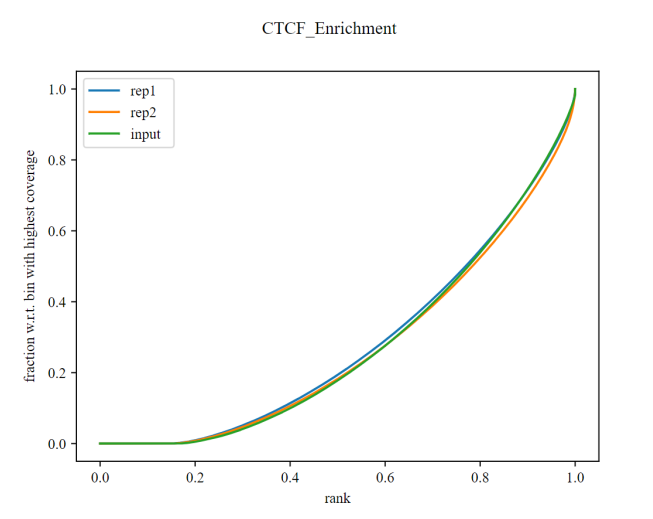
\includegraphics[width=10cm]{figure/chipqc.png}
\end{figure}

理论上,对于没有富集的对照组,其累计曲线应接近与对角线,这与我们的结果符合。对于转录因子的强富集,理想的情况下曲线应该会先缓慢上升,到rank较高的区域后再急剧上升,这表明大量的reads分布在较少的特定窗口中,即蛋白质的结合位点存在显著富集。\par
然而本实验中实验组和对照的累计曲线却相当接近,我们并没有进一步向下探索造成这种现象的原因。


\subsubsection{寻峰}
CTCF是一种转录因子,针对CTCF的ChIP-Seq能够将与之有相互作用的DNA片段富集起来。 Peak calling 是一种ChIP-Seq特有的分析流程,用于鉴定基因组中reads的富集部位。
在ChIP-Seq实验中,比对文件reads的分布是链不对称的:reads以转录因子结合位点为中心,在正义链和反义链各自的5’端形成富集。\par
本流程使用MACS(基于模型的ChIP-Seq分析,Model-based analysis of ChIP-Seq)进行call peak分析。\par
该软件假设DNA上的片段在随机状态下服从泊松分布,macs2根据不满足泊松分布的地方寻找富集点。


\begin{lstlisting}
    ##### step5 call peaks ##########

    echo "call peaks started at $(date)"

    ## 将实验组数据提取出来
    cp rawdata/config rawdata/config2
    cat rawdata/config2 | sed "/input/d" > rawdata/config2

    ## 寻峰,对实验组的所有已经过滤、去重、索引的bam文件寻峰
    cat rawdata/config2 | while read id
    do
    macs2 callpeak -t ./03\_mapping/${id}\_filtered\_dedup.bam \
    -c ./03\_mapping/ctcf\_chip\_input\_filtered\_dedup.bam \
    -f BAMPE -g hs -n CTCF\_ChIP -B -q 0.01 \
    --outdir ./05\_peak\_calling > $./05\_peak\_calling/peak\_calling.log 2>&1
    done
    echo "call peaks finished at $(date)"

    ### 参数说明
    ### -t 处理组的比对文件
    ### -c 对照组的比对文件
    ### -f 输入文件的格式, 设为auto则表示自动识别输入文件的格式;双端测序用BAMPE
    ### -g 有效基因组大小,hs表示人的有效基因组大小,约为2.7E9
    ### -n name string,会成为输出文件的prefix
    ### --outdir 输出文件路径
    ### -B/--BDG 保存堆积对齐片段到bedGraph文件里
    ### -q FDR Cutoff

    ## 备注
    # broad peak常用于组蛋白修饰的peak calling,因为组蛋白修饰往往是一大片;用另外一个程序来call peak
    # narrow peak用于转录因子的peak calling,因此本课题应该使用narrow peak calling。
    # narrowPeak 也可以放进igv里
\end{lstlisting}
macs2的输出结果如下:
\begin{figure}[ht]
    \centering
    \includegraphics[width=7cm]{figure/macs2\_output.PNG}
\end{figure}

NAME\_peaks.xls保存了每个peak的信息:

\begin{enumerate}
    \item chromosome name:染色体名
    \item start position of peak:peak开始的位置
    \item end position of peak:peak结束的位置
    \item length of peak region:peak区域的长度
    \item absolute peak summit position:peak峰出现的位置
    \item pileup height at peak summit:peak峰的堆积高度
    \item -log10(pvalue) for the peak summit (e.g. pvalue =1e-10, then this value should be 10)
    \item fold enrichment for this peak summit against random Poisson distribution with local lambda:相对于随机选取的片段,peak峰高度的变化倍数,即富集倍数
    \item -log10(qvalue) at peak summit
\end{enumerate}
NAME\_peaks.narrowPeak也同样储存了peak的信息:
\begin{enumerate}
    \item 1;染色体号
    \item 2:peak起始位点
    \item 3:结束位点
    \item 4:peak name
    \item 5:int(-10*log10qvalue)
    \item 6:正负链(如果不区分,则记为".")
    \item 7:fold change
    \item 8:-log10pvalue
    \item 9:-log10qvalue
    \item 10:peak的峰相对于peak的位置
\end{enumerate}
NAME\_summits.bed文件记录了所有peak峰的位置和可信度,下游可进一步利用该文件寻找motif\par
NAME\_treat\_pileup.bdg文件用于存放区间的坐标轴信息和相关的评分文件,用于储存稀疏,不连续的数据,并可转化为bigwig文件(二进制,有索引,更高效)\par
NAME\_control\_lambda.bdg文件记录了由对照组中估计得到的局部偏好,可转化为bigwig文件。\par
下载igv软件后,可将排序并索引后的bam文件与narrowPeak文件导入IGV进行可视化查看。
\begin{figure}[ht]
    \centering
    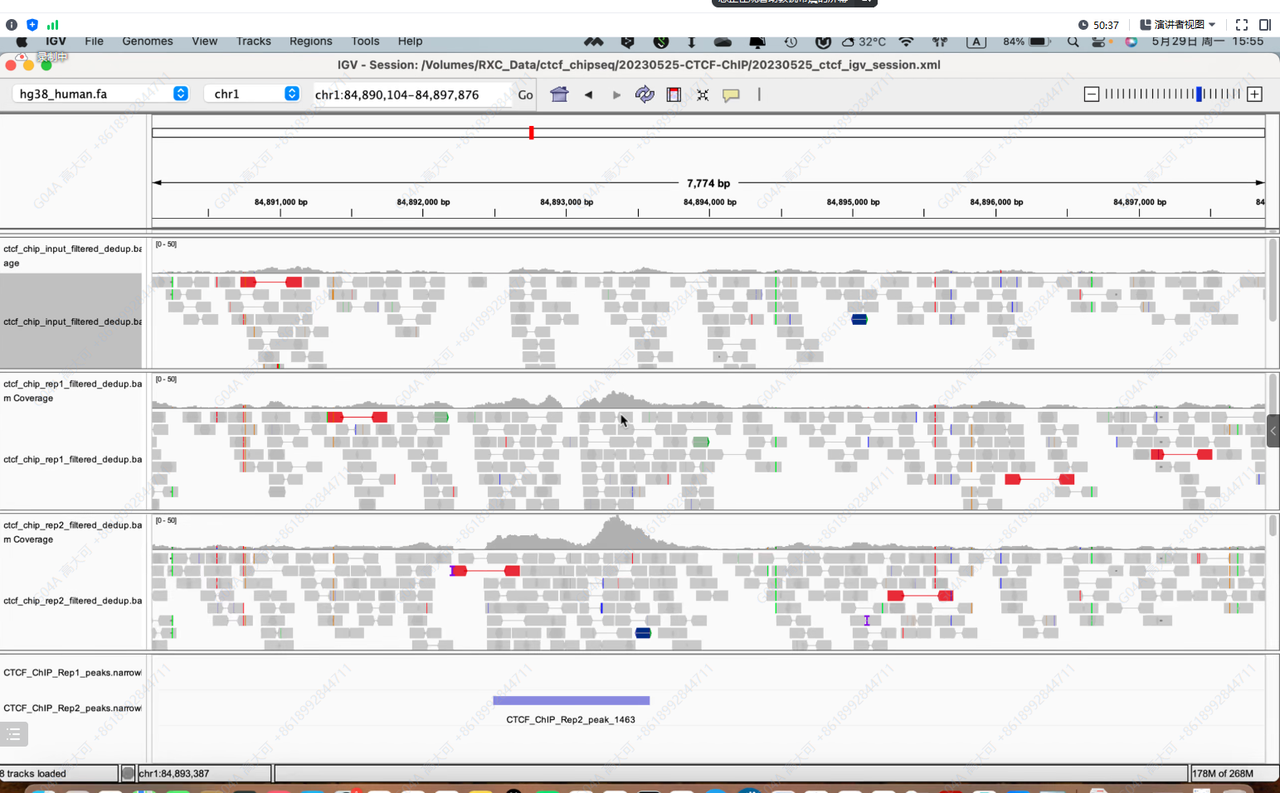
\includegraphics[width=13cm]{figure/igv.png}
\end{figure}

从上图中我们可以可视化地看见narrowpeak的位置,以及那些染色体位置上存在峰的富集。从该图中还能看见部分read太长,只测得了两端(这种情况下macs2会用-f BAMPE进行矫正),部分read太短,二代测序将其测穿,部分位点存在PCR错配或SNP。\par
如果仔细对比rep1和rep2的bam文件在IGV上的可视化图像,可以发现,有的reads的富集在rep2上明显比rep1更多,这可能是因为建库时rep2的富集效果更好,或rep1中某些reads的质量不满足被清洗掉了,或者没有通过假设检验,可以尝试将q值从0.01提高到0.05。\par


\subsubsection{生物学重复的合并}
在进行下游分析时,可以将生物学重复样本合并后进行分析。可以使用IDR软件评估生物学重复样本的相关性,并根据阈值筛选出最终的一组peak,即该软件可从多个生物学重复样本的peak结果中提取高一致性peak区间。\par
使用idr前首先需要对MACS2的结果文件narrowPeak按照p-value排序;排序完成后进行合并。

\begin{lstlisting}
    cat rawdata/config2 | while read id
    do
    sort -k8,8nr ./05\_peak\_calling/${id}\_peak.narrowPeak > ./05\_peak\_calling/${id}\_sorted\_peaks.narrowPeak 
    done

    ### -k8,8 选项使输入文件按其第八列进行排序
    ### -nr 选项指定按整个数字排序(而非一个字符一个字符去比较)

    idr --samples ctcf\_rep1\_sorted\_peaks.narrowPeak ctcf\_rep2\_sorted\_peaks.narrowPeak --input-file-type narrowPeak --rank p.value --output-file sample-idr --plot --log-output-file sample-idr.log
    ### --samples: narrowPeak的输入文件(生物学重复样本)
    ### --input-file-type: 输入文件格式为narrowPeak
    ### --rank p.value: 指定输入文件以p.value排序的
    ### --output-file: 指定输出文件路径
    ### --plot: 输出IDR度量值的结果
\end{lstlisting}

输出文件中,sample-idr是共有peaks的结果输出文件。包含了整合后结果与原本样品1和2的信息。sample-idr.png是结果输出图,描述了两个生物学重复样本中峰的保留情况。\par
在项目的后续分析中没有使用合并的样本,只使用了rep1进行后续下游分析。

\section{ChIP-Seq下游分析}
\subsection{call motif}
使用meme套件进行该任务。\par
可以使用meme-chip寻找motif,并可以详细查看某个转录因子的信息。

\begin{lstlisting}
    mkdir 06\_downstream


    ##### step6. call motif, peak注释和motif search ########

    prefix=CTCF\_ChIP # 该prefix与peak calling的prefix相同
    ### 首先提取用于寻找motif的fasta文件
    ## 取峰值前后100个碱基,第二列-50得到第六列,第三列+49得到第七列,print第1(染色体列),6,7,4列
    awk -v OFS="\t" '{$6=$2-50;$7=$3+49;print $1','$6','$7','$4}' ./04\_peak\_calling/${prefix}\_summits.bed > ./06\_downstream/${prefix}\_motif.bed
    bedtools getfasta -fi /home/wuhangrui/database/ref/hg38/GRCh38.p13.genome.fa -bed ./06\_downstream/${prefix}\_motif.bed > ./06\_downstream/${prefix}\_motif.fasta

    cd /home/wuhangrui/practice/chipseq/06\_downstream

    echo "calling motif started at $(date)"

    mkdir memechip\_out

    meme-chip -db /home/wuhangrui/database/motif\_databases/HUMAN/HOCOMOCOv11\_full\_HUMAN\_mono\_meme\_format.meme -meme-p 10 -dna ${prefix}\_motif.fasta -oc /home/wuhangrui/practice/chipseq/06\_downstream/memechip\_out

    echo "calling motif finished at $(date)"
    cd /home/wuhangrui/practice/chipseq
\end{lstlisting}

可以在输出文件夹下找到输出结果html文件,meme-chip中可以看到软件找出的motif,点击后可在tomtom页面看到该motif的详细信息。\par
注意html结果文件必须和其他meme-chip的输出文件在同一目录下。
\begin{figure}[ht]
    \centering
    \begin{minipage}[c]{0.9\textwidth}
        \centering
        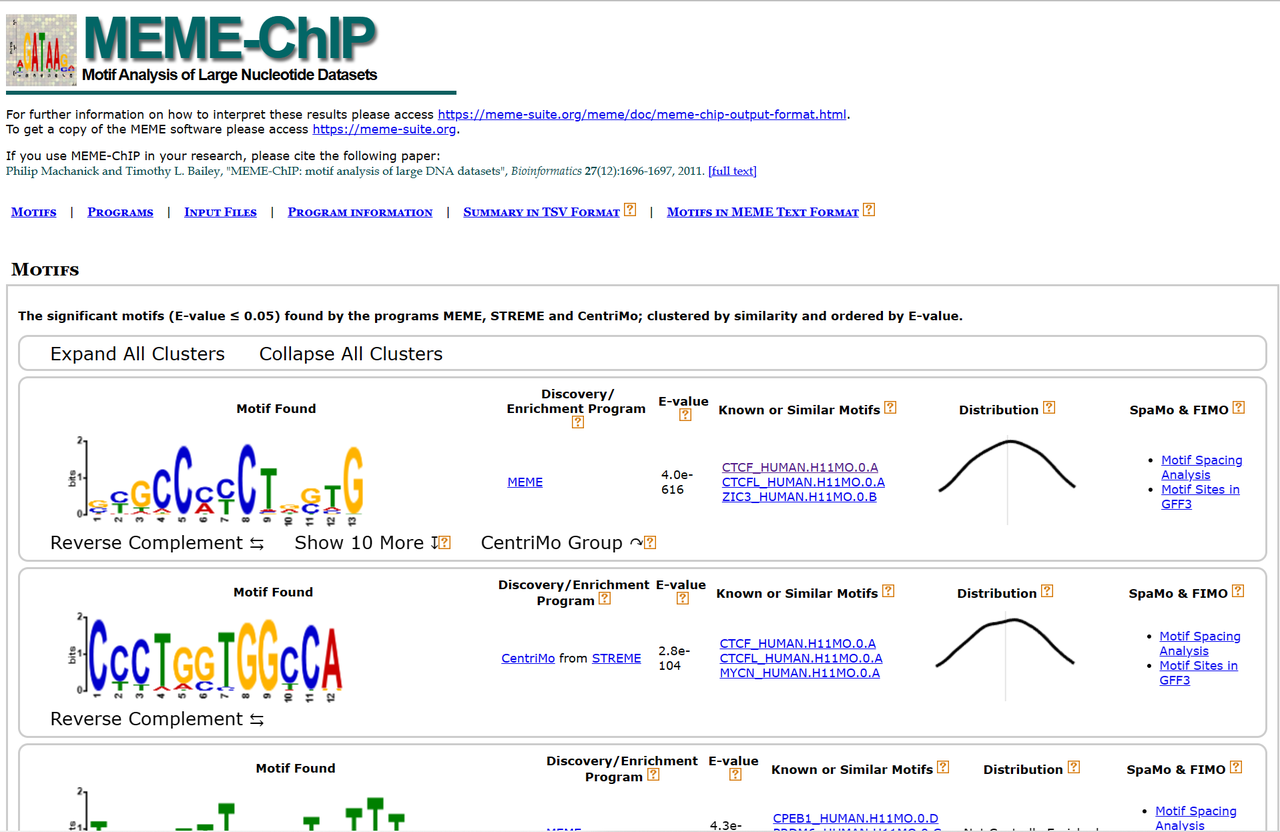
\includegraphics[width=13cm]{figure/memechip.png}
    \end{minipage}

    \begin{minipage}[c]{0.9\textwidth}
        \centering
        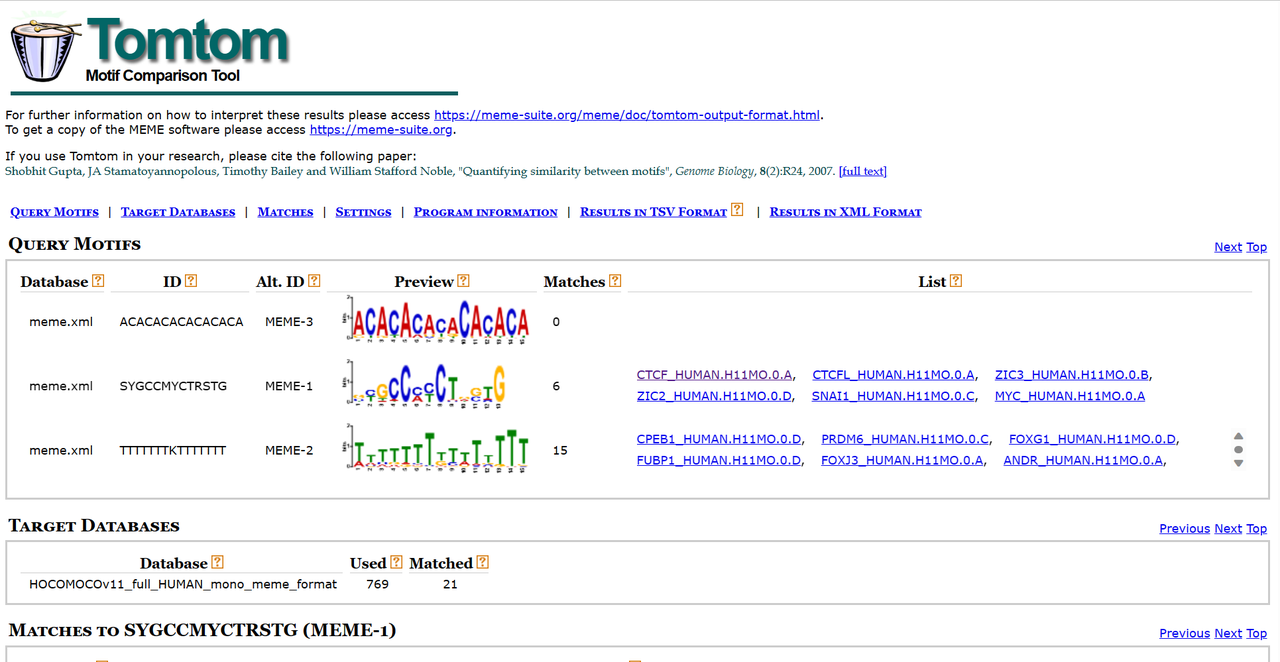
\includegraphics[width=13cm]{figure/tomtom.png}
    \end{minipage}
\end{figure}

\subsubsection{peak注释}
使用Homer进行Peak的注释。Homer包含一个用于峰注释的程序annotatePeaks.pl。它可以将峰与其他附近的基因关联起来。\par
annotatePeaks.pl在默认情况下,会寻找距离peak最近的TSS,并根据TSS所属的基因进行注释。此外该脚本还会根据peak占据的位置,注释其基因组信息
\begin{lstlisting}
    ##### step7. peakannotation ##########
    cd /home/wuhangrui/practice/chipseq/06\_downstream

    echo "peak annotation started at $(date)"
    mkdir peak\_annotation
    annotatePeaks.pl /home/wuhangrui/practice/chipseq/04\_peak\_calling/${prefix}\_peaks.narrowPeak hg38 > peak\_annotation/peak\_annotation.tsv
    echo "peak\_annotation finished at $(date)"

\end{lstlisting}
注释peak得到的信息是表格形式,不方便查看和进一步研究。可以将该输出文件下载到本地用,使用R进行可视化。例如ChIPseeker,GO富集分析,KEGG富集分析等。
该部分是得到的peak注释的进一步分析,和linux本身关系不大,此处省略该部分的代码。可在本组github仓库上寻找相关代码。

\subsection{计算与TSS的共定位情况}
\begin{enumerate}
    \item TSS bed文件可UCSC网站上直接下载,下载选项只需要5’UTR的位置
    \item 需要将索引好的BAM文件转化为bigwig文件
    \item 使用deeptools包下的软件完成该项任务
\end{enumerate}
\begin{lstlisting}
    ##### step8. 不适合看motif的共定位分析 #######
    ##### 8.1 与TSS, TES的共定位情况 #####
    # 使用bamCoverage进行 bam -> bigwig 文件转换(一种压缩方式:将基因组压缩为很多个bin区域)
    # bigwig 文件记录的是“每个碱基”的coverage情况,可以理解为ChIP-Seq的信号
    # 实验组对照组都需要此步骤

    cd /home/wuhangrui/practice/chipseq/06\_downstream
    mkdir co\_location

    # 将input和rep1都进行bam -> bw 文件的转换

    cat /home/wuhangrui/practice/chipseq/rawdata/config | while read id
    do
    bamCoverage --bam /home/wuhangrui/practice/chipseq/03\_mapping/${id}\_filtered\_dedup.bam \
    -o ./co\_location/${id}\_filtered\_dedup.bw \
    --binSize 10 \
    --normalizeUsing RPGC \
    --effectiveGenomeSize 2913022398 \
    --extendReads \
    -p 10
    done

    ### --bam输入的bam文件
    ### -o 输出的bigwig文件
    ### --binSize 计算coverage时的bin的大小
    ### --normalizeUsing 选择normalization的方法 RPGC按照bin和测序量大小归一化
    ### --effectiveGenomesize 如果需要normalization则需有设置有效基因组大小
    ### --extendReads 设置该值以拓展reads的长度,以计算出用于测序的DNA片段的长度;pair-end的测序可以自动估计DNA片段的长度
    ### -p 使用的线程数


    ##### 与其他区域的共定位情况(高甲基化区域,低甲基化区域,5'UTR,3'UTR等)
    # 使用“computeMatrix”计算指定位置的信号矩阵
    cd /home/wuhangrui/practice/chipseq/06\_downstream

    computeMatrix reference-point \
    -S ./co\_location/ctcf\_chip\_input\_filtered\_dedup.bw ./co\_location/ctcf\_chip\_rep1\_filtered\_dedup.bw ./co\_location/ctcf\_chip\_rep2\_filtered\_dedup.bw \
    -R /home/wuhangrui/database/ref/hg38/uscs\_refseq.bed \
    -a 2500 -b 2500 \
    --samplesLabel input ctcf\_rep1 ctcf\_rep2 \
    --sortRegions descend \
    -o ./co\_location/Rep1\_Input\_TSS\_Matrix.gz \
    -p 10 > computeMatrix\_input.log 2>&1

    # 使用reference-point模式,reference位点为TSS位置
    ### -S 输入的bigwig文件
    ### -R 记录reference位点信息的bed文件
    ### -a 起始位点上游的距离
    ### -b 起始位点下游的距离
    ### --sortRegions 在矩阵中,信号按什么顺序排列?
    ### --samplesLabel 在矩阵中,样品如何命名
    ### -o 输出的矩阵名
    ### -p 线程数
    ### 如果热图中出现黑色条状色块,可以尝试增加--missingDataAsZero选项

    # 使用plotHeatmap作图
    cd /home/wuhangrui/practice/chipseq/06\_downstream
    plotHeatmap -m ./co\_location/Rep1\_Input\_TSS\_Matrix.gz \
    -out ./co\_location/Rep1\_Input\_TSS\_Matrix.svg \
    --plotFileFormat svg --yAxisLabel RPGC --regionsLabel all\_tss \
    --legendLocation none

    ### -m 输入的矩阵文件
    ### -out 输出的图片文件
    ### --plotFileFormat 指定输出文件的格式
    ### --yAxisLabel 指定y轴标签
\end{lstlisting}

\begin{figure}[ht]
    \centering
    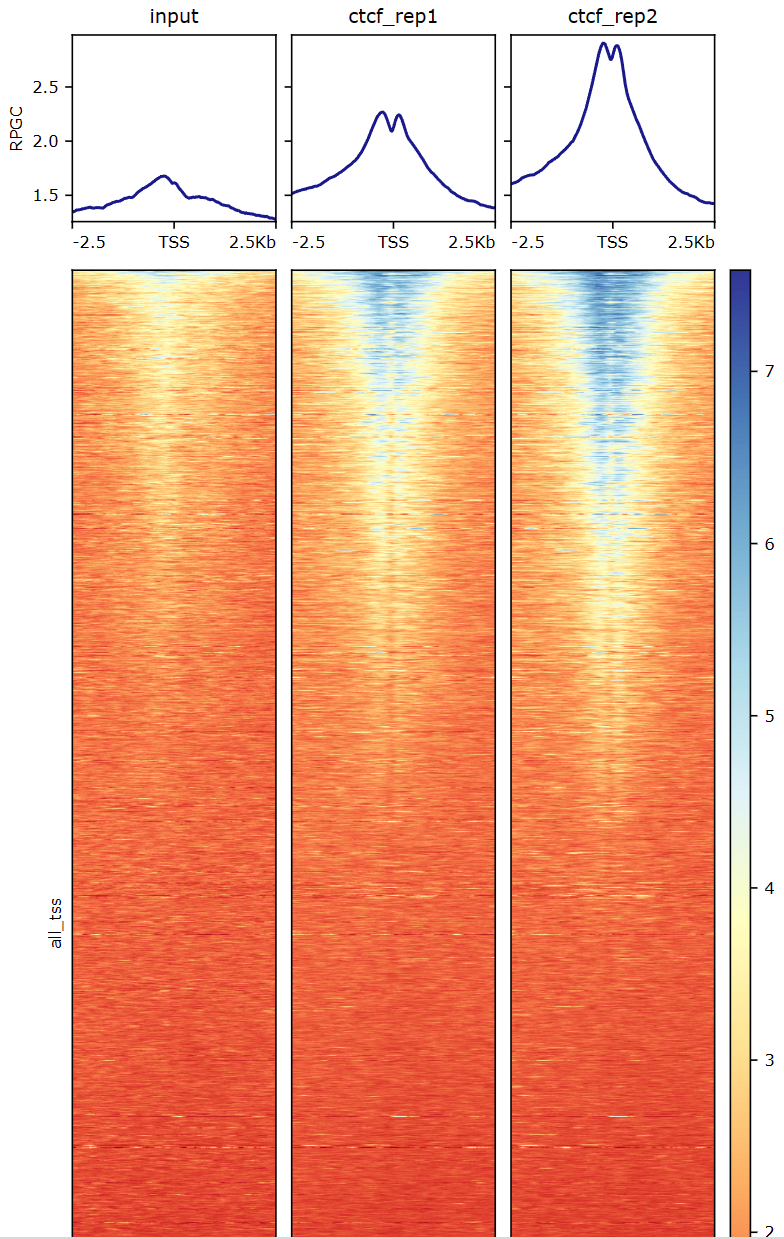
\includegraphics[width=13cm]{figure/heatmap.png}
    \caption{热图}
    \label{heatmap}
\end{figure}

如图\ref{heatmap},可见处理组在TSS上有非常明显的富集,且呈现双峰模式。颜色表示reads密度。